\documentclass[10pt, a4paper]{article}
\usepackage{lrec2006}
\usepackage{lingmacros}
\usepackage{graphicx}
\usepackage[utf8]{inputenc}

\title{Combining Language Resources Into A Grammar-Driven Swedish Parser}

\name{Malin Ahlberg, Ramona Enache}

\address{ Department of Computer Science \& Engineering\\
          Gothenburg University \\
          Box 8718, SE-402 75 Gothenburg, Sweden\\
          ahlberg.malin@gmail.com, enache@chalmers.se \\}

%TODO check ref-list

% 150-200 words here
\abstract{This paper describes work on a rule-based, open-source parser for
Swedish. The central component is a wide-coverage grammar implemented in the GF
formalism (Grammatical Framework), a dependently typed grammar formalism
based on Martin-L{\"o}f type theory. GF has strong support for multilinguality and
has so far been used successfully for
controlled languages \cite{cnl}. Recent experiments have showed
that it is also possible to use the framework for parsing unrestricted language.
In addition
to GF, we use two other main resources: the Swedish treebank Talbanken and the
electronic SALDO lexicon. By combining the grammar with
a lexicon extracted from SALDO we obtain a parser accepting all sentences
described by the given rules. We develop and test this
on examples from Talbanken.
The resulting parser gives a full syntactic analysis of the input sentences.
It will be highly reusable, freely available, and as GF provides libraries for
compiling grammars to a number of programming languages, chosen parts of the the 
grammar may be used in various NLP applications. 
\\ \newline \Keywords{GF, Swedish, Parsing, Computational Grammar, Lexical Acquisition}}

\begin{document}

\maketitleabstract


% TODO add links to the website?
\section{Introduction}
Our goal is to implement a wide-coverage grammar and parser for Swedish
using the GF formalism, and 
thereby investigate how GF can be used for open-domain parsing.
We compile a large-scale grammar to a parser
and combine it with the extensive lexicon SALDO. The Swedish treebank 
Talbanken provides manually tagged trees which we use for improving and evaluating
the grammar. The parser will additionally
be evaluated by an expert. \\
We chose our resources so that both our grammar and parser can 
be freely available and open-source. 
The target language is Swedish, a North-Germanic language
closely related to Norwegian and Danish. The languages share most of their
grammatical structures and are mutually intelligible. Swedish is also 
one of the official languages in Finland and altogether spoken by approximately 9
million people.
Swedish syntax is often similar to English, but the  morphology is richer and the
word order slightly more intricate.
It is a verb-second language: the second constituent of a declarative main
clause must consist of a verb.
The first constituent of the clause is usually made up of the subject,
although it likewise could consist of adverbial phrases or objects.
Fronting the finite verb marks questions.

This paper will briefly introduce GF, Talbanken and SALDO in Section \ref{sec:background}
Section \ref{sec:extractsaldo} explains how we extract a lexicon, section \ref{sec:mapping}
how we translate Talbanken to GF annotation and section \ref{sec:grammar}
presents the work on the grammar implementation.


\section{Background}
\label{sec:background}
\subsection{Grammatical Framework}
\label{sec:gf}


Grammatical Framework \cite{ranta-2011} is a grammar formalism based on
functional programming. 

The key idea is to divide a grammar into abstract and concrete parts. 
The abstract grammar gives a logical representation of the semantics,
modeled as abstract trees.
The concrete grammars tell how to translate the abstract trees to a given language,
and deal with issues such as word order, case and agreement. 
The framework enables us to parse strings into abstract trees as well as
linearize trees into strings.

The grammar acts as an independent module and reusability is further supported
by the separation between resource grammars and application grammars. The
resource library provided with GF implements morphological and syntactical
rules for more than 20 different languages.  Hence the writer of an application
grammar can start her work at a higher level and does not need to describe how
to form standard sentences, phrases or inflect words.

Since many of the languages in the GF library resemble each other grammatically,
they can share much of their implementations. This is usually done by using a
\verb|Functor| by which we avoid code duplication and which aids the code maintenance.

GF has so far been used in a number of projects,
MOLTO\footnote{http://www.molto-project.eu/}, TALK \cite{talk}
and WebAlt \cite{webalt} to mention a few. 
All those are special domain applications, dealing with controlled natural
language.
This project takes a different approach by using GF for open domain language,
similar to the recently conducted work on translation of patents \cite{patent}.

Using the Swedish resource grammar as our starting
point, we get a basic description of the language. The framework provides
tools such as parsing, generation and
a well-tested interpretation of the parse trees. Furthermore, there are tools
for using GF grammars in a number of programming languages like Haskell
and Java. 



\subsection{Talbanken}
For development and evaluation, we use the Swedish treebank
Talbanken \cite{talbanken}.
It was assembled in the 1970s at Lund University and later
%in 2005 \cite{talbanken05} and
enriched with annotation for a full phrase structure analysis \cite{talbanken05}.  \\
Although Talbanken contains both written and spoken Swedish,
only the prose material, consisting of 6316 sentences, is used in this
project.
This part was also used when training the data-driven parser Maltparser \cite{malt}. \\

\subsection{SALDO}
SALDO \cite{saldo} is an open source lexicon resource
based on Svenskt Associationslexikon. It is
developed at Spr{\aa}kbanken at Gothenburg University
and intended for usage in language technology
research. 
We have developed tools for extracting GF lexicons
from SALDO, described in section \ref{sec:extractsaldo}

\section{Related work}
% Add: detaild comparison of outputs of various parsers of Sw.
Many years of research have lead to many interesting language
technology tools for Swedish.
An example is the well-known data-driven Malt parser \cite{malt},
trained on Talbanken. 
There are also a number of grammar-based parsers, although none is freely available.
The cascaded finite state parser CassSwe \cite{casswe} and
The Swedish Constraint Grammar \cite{birn}
give syntactic analyses. 
Swedish FDG (Voultanien,2001) uses the Functional Dependency Grammar
\cite{fdg},
an extension of the Constraint Grammar
formalism, and produces a dependency structure focusing on finding the nominal
arguments. \\
The LinGO Grammar Matrix \cite{matrix}, is a starter-kit for building
Head-Driven Phrase Structure Grammars \cite{hpsg} (HPSG) providing
compatibility with tools for parsing, evaluation, semantic representations etc.
Translation is supported by using Minimal Recursion
Semantics \cite{mrs} as an interlingua. 
There is a collection of grammars implemented in this framework, giving broad-coverage
descriptions of 
English, Japanese and German. 
The Scandinavian Grammar Matrix \cite{scandmatrix} covers common parts of
Scandinavian, while Norsource (Hellan, 2003) describes Norwegian. A Swedish version
was based upon this by Ahrenberg, covering the morphology and some
differences between Swedish and Norwegian. Further, there is the BiTSE 
grammar \cite{stymne}, also implemented using the Lingo Matrix,
which focuses on describing and translating verb frames.\\ 
The Swedish version of the Core Language Engine (CLE) \cite{gamback}
gives a full syntactic analysis as well as semantics represented in `Quasi logical form'. A
translation to English  was implemented and the work was further developed in the spoken
language translator \cite{spoken}. Unfortunately, it is no longer available.\\
%The coverage of the Swedish
%CLE is also reported to be very limited \cite[p. 134]{nivreTrees}.\\
In the TAG formalism \cite{tag}, there are projects on getting open-source, wide-coverage grammars
for English and Korean, but, to our knowledge, not for Swedish.  \\
The ParGram \cite{pargram} project aims at making wide coverage grammars using
the Lexical Functional Grammar approach \cite{lfg}.
The grammars are implemented in parallel in order to coordinate the analyses of
different languages and there are now grammars for English, German, Japanese and Norwegian. 

Extract \cite{MarkusForsberg2007} is a tool for lexicon
%TODO
extraction compatible with GF, sharing its basic ideas with our lexical
acquisition tool. Extract does however not consider parts-of-speech and our
tool is developed closer to GF, while still
having additional mechanisms for being robust and human support to be accurate.


\section{Extracting a large lexicon}
\label{sec:extractsaldo}
The lexicon provided with the GF resources is far too small for open-domain
parsing.
This section describes the process of importing SALDO, which is 
compatible with GF, and easily translated to GF format.
As SALDO is continuously updated, the importing process has been designed to be fast
and stable enough to be redone at any time.

\subsubsection{Implementation}
The basic algorithm for importing SALDO was implemented by Angelov (2008)
and  produces code for a GF lexicon.
For each word in SALDO, it decides which forms should be used as input
to the GF smart paradigms. The smart paradigm is a function which given one
form of a word, can infer which paradigm it most likely belongs to.
For verbs, this will in most cases mean giving
the present tense form, see figure \ref{fig:saldoknyt}. \\

\begin{figure}[h]
\begin{center}
\verb-mkV "knyter" ;-
\caption{First code produced for the verb `knyta' (\emph{`tie'})}
\label{fig:saldoknyt}
\end{center}
\end{figure}

All assumed paradigms are printed to a temporary lexicon, 
which will produce an inflection table for every entry when compiled.
The tables are compared to the information given
in SALDO and if the tables are equal the code for the word is saved. If the table
is erroneous, another try is made
by giving more forms to the smart paradigm.
For example \ref{fig:saldoknyt}, the smart paradigm will fail to calculate the
correct inflection table. In the next try both the present and the past tense
are given:\\

\begin{figure}[h]
\begin{center}
\verb-mkV "knyter" "knöt" ;-
\caption{Second output for the verb `knyta'}
\label{fig:saldoknyt2}
\end{center}
\end{figure}

The program is run iteratively until the GF table matches the one given in SALDO,
or until there are no more ways of using the smart paradigm. The verb 'knyta'
will need three forms:\\

\begin{figure}[h]
\begin{center}
\verb-mkV "knyter" "knöt" "knutit"-\\
\caption{Final output for the verb `knyta'}
\label{fig:saldoknyt3}
\end{center}
\end{figure}


\subsubsection{Results}
\label{sec:saldoRes}
The resulting dictionary contains more than 100 000 entries, approximately 80 \% 
of the total size of SALDO.
There are a number of reasons why some words were not imported,
the most obvious one is that we do not want all categories from
SALDO in the GF lexicon. Prepositions, 
numerals, 
personal pronouns etc.
are assumed to be present in the resource grammars and should not be added again.
SALDO contains many pronouns which
are not analyzed the same way in GF. 
Before adding them to our lexicon, we need to do more analyzing to find their
correct GF-category. 
Categories involving multiple words 
are usually handled as idioms and should be given in a separate lexicon. In
total six types of words were considered for the extraction: \\

\begin{figure}[h]
\begin{tabular}{|l|ll|}
\hline
& SALDO$/$GF & Example \\
\hline
 Adverb & \textbf{ab}$/$\textbf{Adv} & ofta (\emph{often})\\
 Adjective&\textbf{av}$/$\textbf{A} & gul (\emph{yellow})\\
 Noun & \textbf{nn}$/$\textbf{N} & hus (\emph{house})\\
 Verb & \textbf{vb}$/$\textbf{V} & springa (\emph{run})\\
 Reflexive verbs &\textbf{vbm}$/$\textbf{V} & raka sig (\emph{shave})\\
 Particles verbs &\textbf{vbm}$/$\textbf{V}  &  piggna till (\emph{perk up})\\
\hline
\end{tabular}
\caption{}
\end{figure}

Most but not all words of these categories have been imported.
One reason why the importing phase would fail 
is that SALDO, unlike GF, only contains the actually used word forms.
For technical reasons, the smart paradigm might need forms never used.
Consider for example the plural tantum 
noun \emph{`glas{\"o}gon'} (\emph{`glasses'}).
The smart paradigm requires a singular form, and since the program could not
find this in SALDO, there was no way of adding the lemma to the lexicon. 
When the program failed to import a noun, this was often the explanation.
Words of this type may be added manually, for \emph{`glas{\"o}gon'} we could use
the ostensibly correct singular form `glas{\"o}ga', although this
has another meaning (`glass-eye').
The same problem occurred for the irregular s-verbs,
(\emph{`synas'} \emph{(`show')} or \emph{umg{\aa}s} \emph{(`socialize')})
which made up 61.5 \% of the failing verbs of type \verb_vb_.\\
In a few cases the smart paradigms could not generate the correct declination.\\
When testing the coverage of Talbanken,
we found that there are around 2500 word forms still missing, excluding the ones
tagged as names and numbers. This number may seem very high, but 
4/5 of the word forms are compounds and when performing the intended parsing,
an additional analysis identifying compounds is preformed before
looking-up the words in the lexicon. 
Talbanken also contains a small number of 
spelling errors, which probably are enumerated among our missing words. The majority
of the missing words are only used once.\\
\begin{figure}[h]
\begin{tabular}{|l|l|}
\hline
Missing words &$\sim$ 2500 word-forms\\
\hline
\hline
Ignoring compounds & $\sim$ 500 word-forms\\
Used more than once & $\sim$ 500 word forms\\
Used more than once,& \\
\hspace{2mm} ignoring compounds & $\sim$ 150 word-forms\\
\hline
\end{tabular}
\caption{}
\end{figure}
A list of words that were given different labels in GF than in Talbanken has been
composed, consisting of about 1600 entries. Many of those are
acceptable and reflects the difference 
made in the analyses, while
others are examples of words that are still missing from
the lexicon.

Valency information, which is crucial for GF, is not given in SALDO and
hence not in the imported lexicon. Instead we are working on methods
of extracting this from
Lexin\footnote{http://spraakbanken.gu.se/lexin/}.


\subsection{A tool for lexical acquisition}
As we extract our main lexicon from SALDO, we have also created a tool for
semi-automatic acquisition to complement the lexicon.
Like the SALDO importer it makes use of
the smart paradigm given in the Swedish resource grammar.
Unlike the SALDO importer, this tool does not require any particular
word form, but operates on any verb form and 
iteratively tries to figure out how to conjugate each of them. If several forms
of a word are 
given, the program will try to identify the one that carries the most linguistic
information, put this in a form recognized by the smart paradigm and ask GF to output
a table with the resulting inflection. 
If the table contains all other conjugations from the input list,
the program will ask the  user to
validate the claimed paradigm. 
This step is needed since the input may not provide information enough
to automatically do the validation. The user may now either
allow the word to be added to the lexicon, remove it or request another guess.
The user hence only needs to decide if each paradigm is correct or not, and
the program will do the rest.

%TODO 
%our largest set of testdata came from talbanken, about 2000? words. Not to large,
%could be better if more forms appeared more often.
The tool has been tested on verbs. Although using simple techniques it 
manages to assign the correct paradigm to 70-75 \% of the given lemmas.
A smaller test has shown that out of the accepted lemmas, the correct guess is
made directly in 75\% of the cases, whereas the user has to reject one or more
guesses for 25\%. 
%Hence the program gets a correctness rate of 56 \% if it is
%run without help from the user. This kind of use is however not intended,


%add: ?
%From this a lexicon with about 1000 verbs have been extracted, manually verified.


\section{Mapping of Talbanken trees}
\label{sec:mapping}
The information from the tags in Talbanken can be used for many purposes.
We have developed an automatic transformation of Talbanken trees 
to trees in GF format. The translation makes use of the POS tags as well as
the syntactic information. 
\begin{figure}[h!]
\begin{center}
\hspace{-30mm}
\subfloat{\label{pic:tbtree}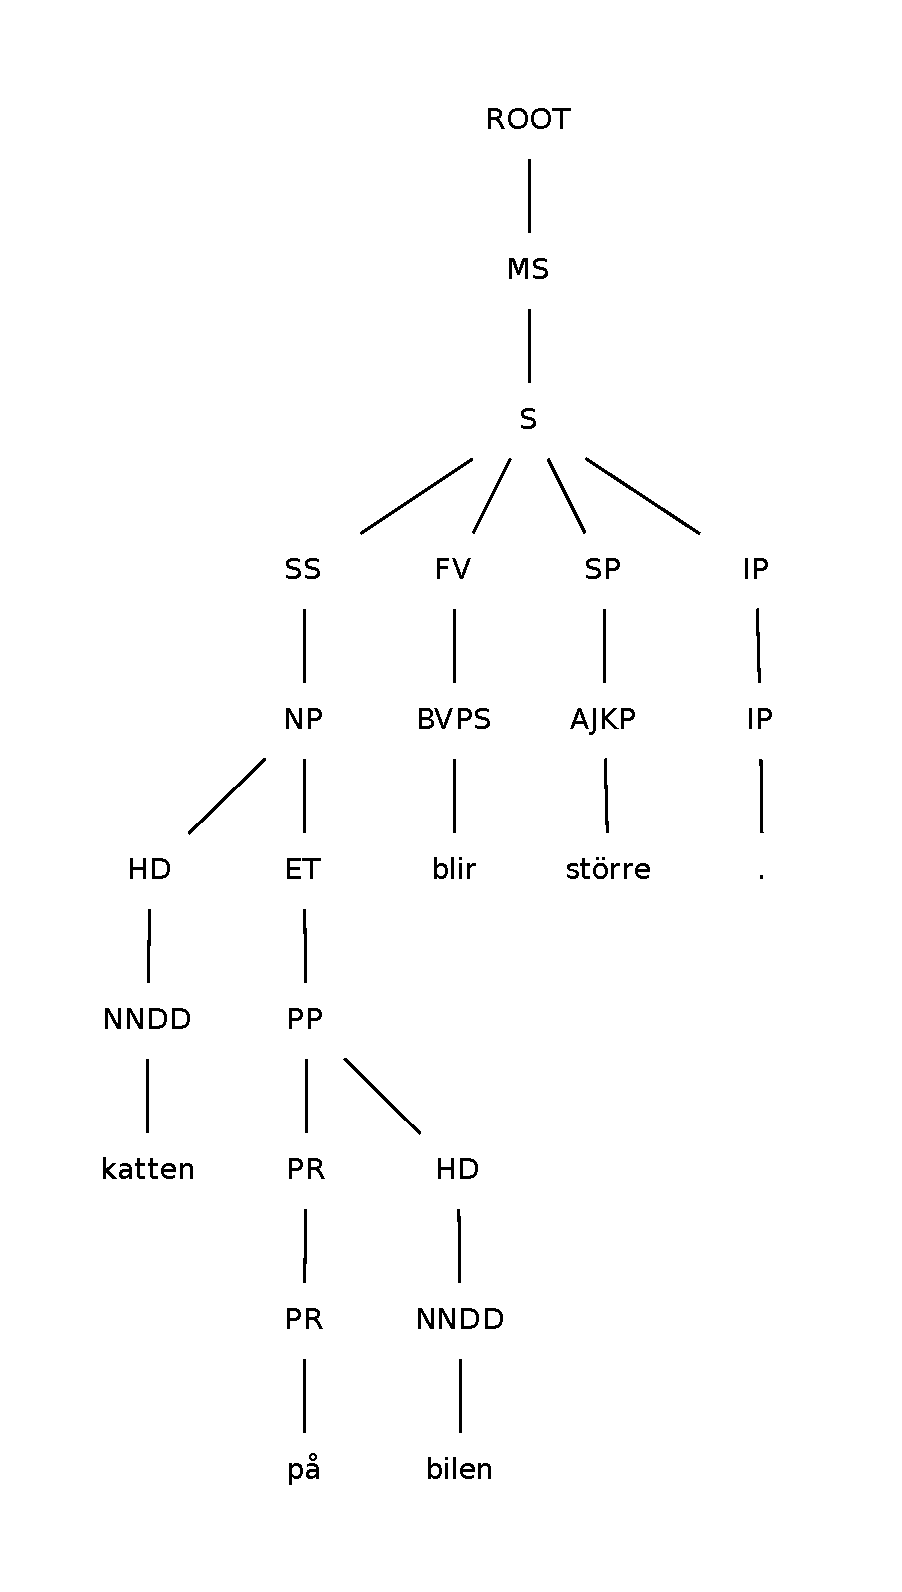
\includegraphics[width=60mm]{Talbankentree.pdf}}
\hspace{-10mm}
\subfloat{\label{pic:gftree}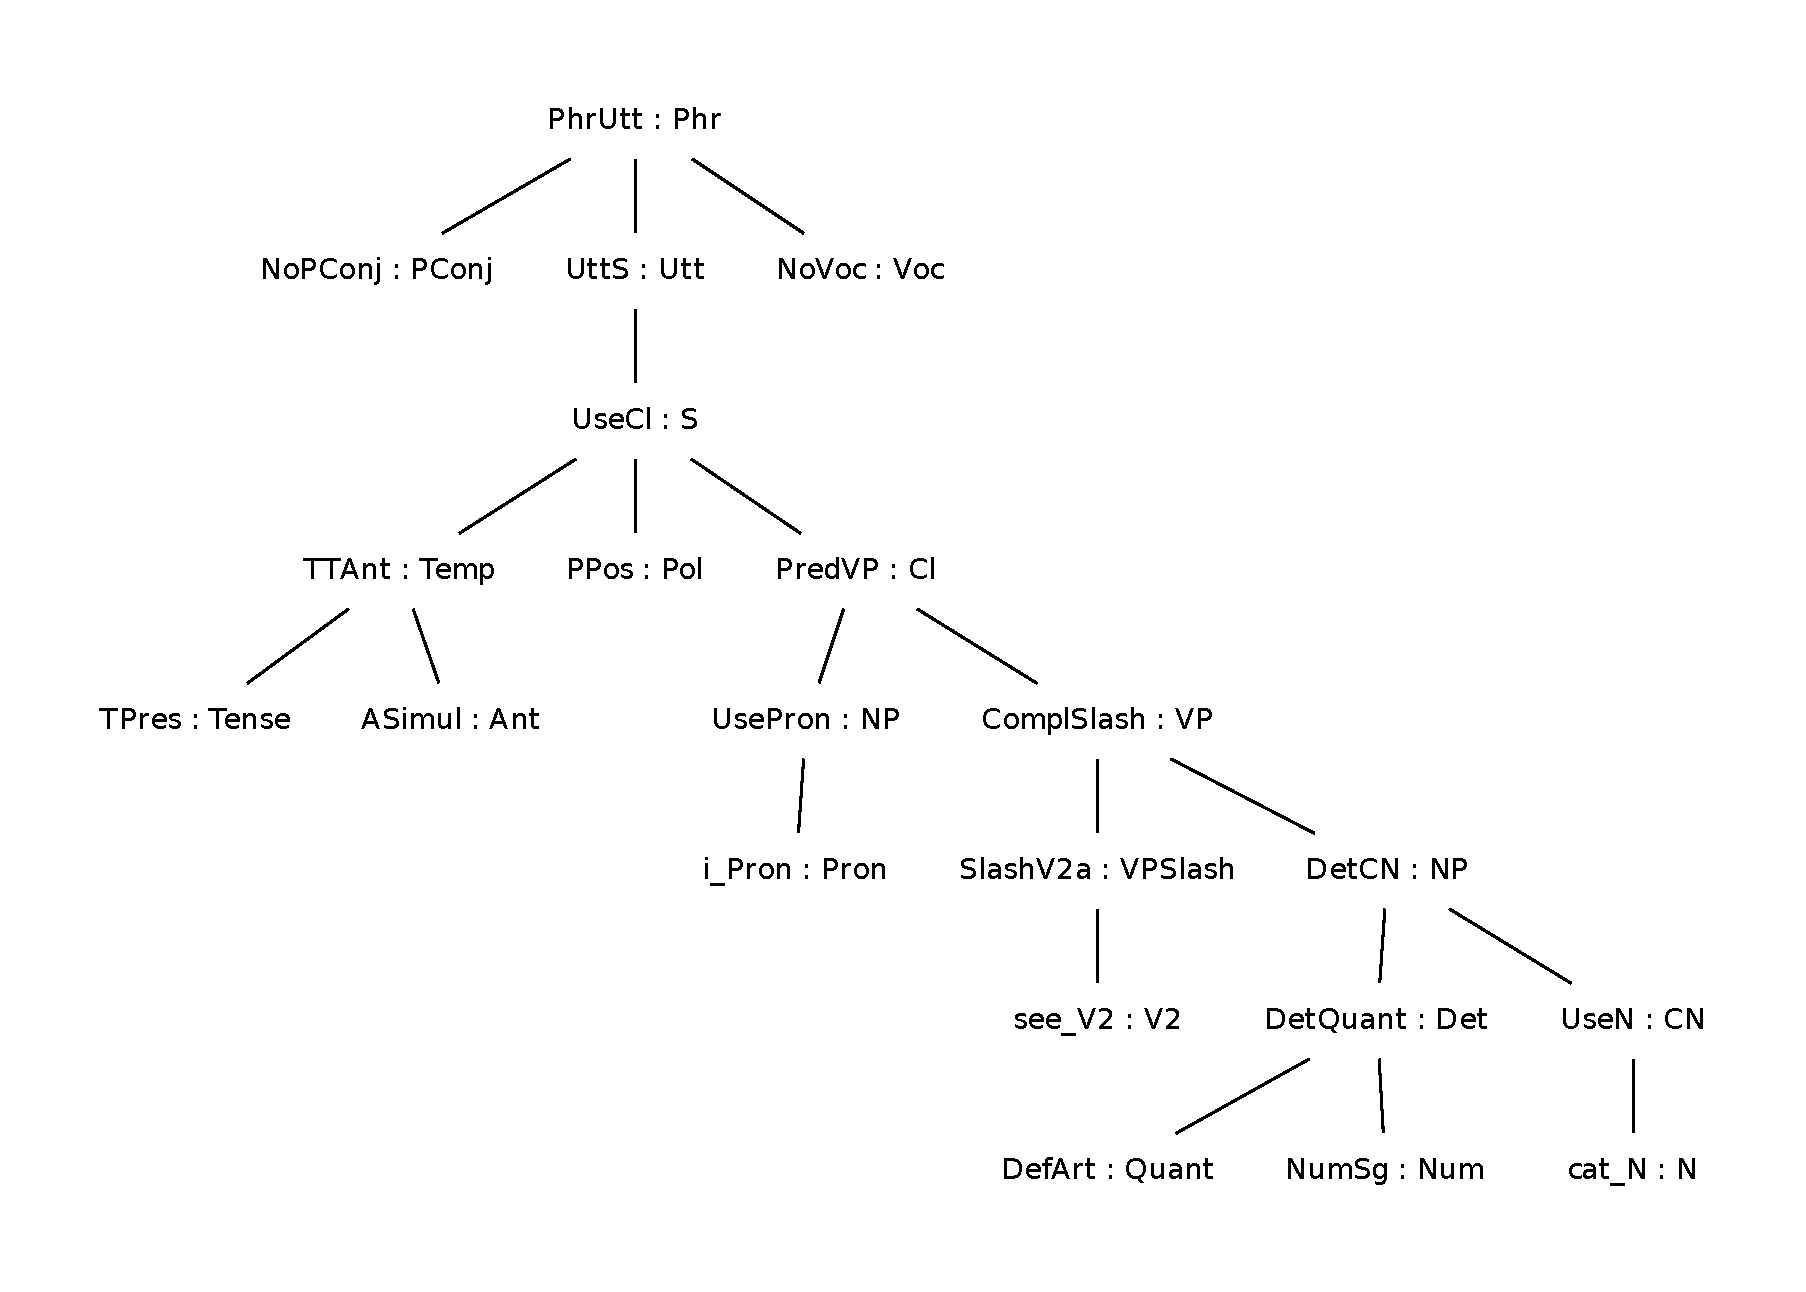
\includegraphics[width=90mm]{gfTree.pdf}}
\caption{The Talbanken tree and the GF tree for the sentence ``Katten p{\aa} bilen blir st{\"o}rre".}
\label{fig:translationtrees}
\end{center}
\end{figure}

Figure \ref{fig:translationtrees} shows an example of a visualized Talbanken05 tree
of the sentence ``Katten p{\aa} bilen blir st{\"o}rre" 
(\emph{``The cat on the car gets bigger"}) and its translation to GF.

The translation 
gives us means to evaluate our parser. By both parsing a Talbanken sentence and
transforming its annotated tree, we can easily inspect if the results are
equal.
Additionally, the mapping shows which grammatical constructions that are still missing
from the GF grammar and shows how the GF analysis differs from the one made
in Talbanken.
If there are words missing from our dictionary, the rich
POS-tags may help us to automatically find the correct declination and add it to the
lexicon. Further, our parser will need probabilities of how often a function is
used. The GF treebank we achieve from the translation is a good source for this
information.\\

\subsection{Results and evaluation}
The development was mostly example-driven, and at least one rule for the translation of
every Talbanken-tag has been implemented.
Shorter sentences, with less than 10 words, have been prioritized in order to
get a coverage of the most fundamental constructions. 

When evaluating the mapping, the results strongly depend on which restrictions we
put on the input. 
One of the reasons why a node cannot be translated, is the 
use of the tags show in figure \ref{fig:mapBadtag}.
The \textbf{PU} tag is used for graphic listings, and not for fluent text.
In our grammar there is naturally no corresponding function; 
the listings are meant for making the text look nice in
folders etc and outside the scope for the grammar itself. The tags \textbf{XX}
and \textbf{NAC} are often used since Talbanken makes a
difference between subject
and object noun phrases.
The analysis of elliptical expression in (\ref{sent:krav})
\enumsentence{F\"or stora krav.\\
``Too high demands."}\label{sent:krav}
contains the tags \textbf{XX} and \textbf{NAC}, since it is not obvious
whether the noun phrase is used as subject or an object.
The tags shown in figure \ref{fig:mapBadtag} occur quite frequently in the treebank and are always translated
to metas, which lowers our result. \\
\begin{figure}[h]
\begin{tabular}{ll}
\textbf{NAC} & Not a constituent\\
\textbf{XP} & Other (non-coordinated) phrase\\
\textbf{DB} & Doubled function\\
\textbf{PU} & List item\\
\textbf{XX} & Unclassifiable part-of-speech\\
\end{tabular}
\caption{Untranslatable tags}\label{fig:mapBadtag}
\end{figure}


The main goal has been to be able to translate shorter sentences, with no
idioms or conjunction.
If we assure that the lexicon contains the correct word class for all lemmas
involved, we
can restore more than 85 \% of the nodes in the original tree.
If we lift all the restrictions excluding the \verb|PU|, we get
65 \% coverage. 
If we test randomly collected sentences that do not contain any of the tags listed
in figure \ref{fig:mapBadtag}, 72 \% can be restored (see figure \ref{tab:mappres})

\begin{figure}[h]
\begin{tabular}{|ll|}
\hline
No list items & 65 \%\\
No special punctuation or bad tags& 72 \%\\
Short sentences with known words & 85 \%\\
\hline
\end{tabular}
%TODO is this correct???
\caption{Number of nodes in each translated tree not put to meta}
\label{tab:mappres}
\end{figure}

\section{Development of the grammar}
\label{sec:grammar}
An important part of this project has been to develop the Swedish GF grammar and
to adapt it to cover constructions used in Talbanken. As a grammar
implementation can never be expected to give
full coverage of a language, we aim for a grammar fragment which gives a deep
analysis of the most important Swedish constructions.
The starting point has been the GF resource grammar and the new implementation is
still compatible with this.

For Swedish, about 85\% of the GF resource code is shared with the other Scandinavian
languages. 
However, if we aim for a deeper and more comprehensive analysis of Swedish,
the implementation of the languages needs to be more independent.
The resource grammar gives a good start and our present grammar 
covers constructions such as declarative sentences, questions, passives,
imperatives, relative clauses, cleft constructions etc.
A number of constructs that are generally not present in other languages and
therefore not given by the resources, have also been added. These include the use of
the reflexive pronoun \emph{sitt}: \\
\emph{Han s{\aa}g \textbf{sitt} hus} $\; \; \; \;$ (\emph{He saw SELF's house}) $\;$ \\
as opposed to \\
\emph{Han s{\aa}g \textbf{hans} hus} $\;$ (\emph{He saw his (another person's) house}) \\
Fronting words or phrases is very common in Swedish and are now allowed by the grammar:\\
\emph{\textbf{Glad} var han inte.} $\;$ (\emph{\textbf{Happy} was he not}). \\
This sort of rephrasing is not given by the resource grammar, since it
has little effect on the logical representation.

\section{Evaluation and Future Work}
The project has so far resulted in
\begin{itemize}
\item a large-scale GF lexicon and a program to redo the importation when needed
\item an extended grammar covering an important part of Swedish
\item a comparison between GF and another annotation
\end{itemize}

Besides being capable of reimporting SALDO, the lexicon extraction program could also
be modified for importing other lexical resources. The only requirement is that
the resource provides inflection tables.

The grammar has been extended and enhanced, and its current status is
a specialized extension of the resource grammar.
Besides parsing, the grammar may well be used for language generation,
which works fast even when using an extensive lexicon.
By the renewed import of SALDO, we have doubled the size of the lexicon and thereby
added many of the commonly used words that were missing from the older
version. This is of course a big improvement.
However, the lexical part still requires some work before it can be made use of.
The lexicon is too big to use with the current techniques as its size exhausts the
the current incremental parsing algorithm. However, new research is being conducted
to improve the GF run-time system.
%TODO can I write that?

When it comes to parsing, we do not get far without robustness.
The grammar in itself is by no means robust, and just one 
unexpected punctuation mark, unknown word
or ellipsis will cause the parsing of the whole sentence to fail. 

Parsing bigger parts of Talbanken would hence give very low results at this stage, 
and a comparison of the results would not be of much value as
there would not be enough material
to do be able to do any interesting analysis.

Without methods for robust parsing, %TODO evaluate??
it is not interesting to talk about coverage, but about the quality and
the ability to scale up, which has so far proved to be good.
We further believe that the presence of a expert in Swedish, professor Elisabet
Engdahl\footnote{http://svenska.gu.se/om-oss/personal/elisabet-engdahl},
has increased the standard substantially.\\
We are currently working on chunk parsing and disambiguation using probabilities
extracted from our translation of Talbanken. We combine this with simple named
entity recognition and compounding analysis. For evaluation, we intend to use
10 \% of Talbanken, chosen so that is does not infer with our test data.

The result will be evaluated both automatically -- by comparing the output of
the translated trees from Talbanken -- and manually by professor Elisabet Engdahl.
She also evaluates the intermediate results.

\section{Conclusion}
We have developed the main components
for a deep Swedish parser; an extended grammar and lexicon and material for
evaluation and disambiguation.
By starting from the GF resource grammar, we got a well-defined system for
describing language. 
We have developed tools for extending the lexicon with words from Talbanken,
and we show how to make use of the information in the manually tagged
treebank.
\\
All parts of the project are open-source and may thus be used in other applications.
The grammar and the lexicon may be beneficial also when working with controlled languages,
as it increases the coverage of the Swedish resource grammar.

The usage of GF allows us to start from
a well-defined system for describing grammar, as well as tools for
parsing.

\section{Acknowledgments}
The work has been funded by Center of Language Technology.
We would also like to give special thanks to Aarne Ranta,
Elisabet Engdahl, Krasimir Angelov, Olga Caprotti, Lars Borin and John Camilleri for their help
and support.

\bibliographystyle{lrec2006}
\bibliography{FinBib}

\end{document}

